\NeedsTeXFormat{LaTeX2e}
%\documentclass[a4paper,10pt,onecolumn,oneside]{book}
\documentclass[10pt]{article}
\usepackage[unicode,colorlinks]{hyperref}
\usepackage{html}
\usepackage{url}
\usepackage{graphicx}
%\hypersetup{unicode=true} % Makes bookmarks work in Russian

% подавление висячих строк
\clubpenalty=10000
\widowpenalty=10000

% убрать переносы слов
\pretolerance=10000

% межабзацный отступ
\parskip=1.2ex


\hypersetup
{
    pdfauthor={Yuri Timofeev tim4dev@gmail.com},
    pdftitle={Webacula v.5.5. Installation Manual},
    pdfkeywords={webacula, manual, install, bacula}
}


\title{
  \Huge{Webacula v.5.5}
  \begin{center}
   \large{Installation Manual}
  \end{center}
}
\author{
  \begin{small}
    Copyright 2007, 2008, 2009, 2010, 2011 
    Yuri Timofeev \htmladdnormallink{tim4dev@gmail.com}{mailto:tim4dev@gmail.com}
  \end{small}
}
%\date{Jan 2011}



\begin{document}



\maketitle
\clearpage

\tableofcontents
\clearpage

\listoffigures
\clearpage

\section{About this manual}
\label{About}

The basic features of Webacula see in README file.

This manual should give you to install or upgrade Webacula installation.

If you find errors or typos please
\htmladdnormallink{send a bug report}{http://sourceforge.net/tracker/?group_id=201199}.

Thanks.



\section{System Requirements}
\label{System Requirements}

To check the installed system packages, run from command line:
\begin{verbatim}docs/check_system_requirements.php\end{verbatim}

\textbf{NOTE}. The successful execution of the script does not indicate that your system is fully ready to work with Webacula.


Webacula also requires:
\begin{itemize}
  \item Bacula 5.0 or later
  \item Zend Framework version 1.10.0 or later
  \item Zend Framework is built with object-oriented PHP 5 and requires PHP 5.2.4 or later with PDO extension active.
        \htmladdnormallink{Please see the system requirements appendix}{http://framework.zend.com/manual/en/requirements.html}
        for more detailed information.
  \item Apache and \texttt{mod\_rewrite}. Or equivalent web-server, for example, nginx and \texttt{ngx\_http\_rewrite\_module}
  \item Installed \texttt{php-gd} package
  \item Installed \htmladdnormallink{http://php.net/dom}{http://php.net/dom} for use the RSS feed
  \item Browser compatibility: all jQuery UI plugins are tested for IE 6.0+, Firefox 3+, Safari 3.1+, Opera 9.6+, Google Chrome
\end{itemize}



\section{Install}
\label{Install}



\subsection{Make directory tree}
\label{Install:Make directory tree}

Login as root and make directory \texttt{/var/www/webacula} (for example).
Copy Webacula distribution to this directory.

\htmladdnormallink{Download minimal Zend Framework package}{http://framework.zend.com/} and extract.
Copy the contents from directory \\
\texttt{ZendFramework-*-minimal/library/Zend} \\
to \\
\texttt{webacula/library/Zend}

\textbf{NOTE}. If you use the Zend Framework for multiple sites, then you can place it in a folder that is part of
your PHP include path. By doing this, you will have access to the Zend Framework components in all PHP scripts.

The tree which should turn out as a result :

\begin{verbatim}
/var/www/webacula/
|-- application
|   |-- controllers
|   |-- models
|   `-- views
...
|-- data
|   |-- cache
|   |-- session
|   `-- tmp
...
|-- docs
|-- install
|-- html
|-- languages
`-- library
    |-- MyClass
    `-- Zend (here is Zend Framework package)
        |-- Acl
        |-- Auth
        |-- Cache
       ...
\end{verbatim}


Some directory description:

\texttt{application/}    All source code. Should be available to reading for the Web-server and
                  no access through the client Web-browser.

\texttt{html/}    Public code. Should be available to reading for the Web-server and for the client Web-browser.

\texttt{data/}    \textbf{IMPORTANT}. This directory, subdirectory and files in it
                  must NOT be available to access through the client Web-browser.

\texttt{data/cache/}  Cache directory for Zend\_Cache. Should be available to writing the Web-server and
                  no access through the client Web-browser.

\texttt{data/session/}   Storage for PHP session. Should be available to writing the Web-server and
                  no access through the client Web-browser.

\texttt{data/tmp/}   This directory which will be saved the file, which contains a list of files to Job restore.
                  This directory and files in it should be available to read from the Bacula Director and
                  to writing from the Web-server. And no access through the client Web-browser.




\subsection{config.ini}
\label{Install:config.ini}

Specify the parameters to connect to the Catalog database, timezone and other in \texttt{application/config.ini}




\subsection{Setting up to run bconsole under Webacula}
\label{Install:Setting up to run bconsole under Webacula}

Creates system group account (if not yet created) : \\
\texttt{groupadd bacula}

Add apache to group: \\
\texttt{usermod -aG bacula apache}

\textbf{IMPORTANT}. Check \texttt{/usr/sbin/bconsole} it should be the binary ELF file, not a shell script!

Next, setup \texttt{bconsole} can be executed under Apache webserver.



\subsubsection{Without using sudo}
\label{Install:Setting up to run bconsole from under Webacula:without sudo}

\begin{verbatim}
chown root:bacula /usr/sbin/bconsole
chmod u=rwx,g=rx,o=  /usr/sbin/bconsole

chown root:bacula /etc/bacula/bconsole.conf
chmod u=rw,g=r,o= /etc/bacula/bconsole.conf
\end{verbatim}

Edit \texttt{application/config.ini}
\begin{verbatim}
bacula.sudo = ""
bacula.bconsole = "/usr/sbin/bconsole"
\end{verbatim}



\subsubsection{With sudo}
\label{Install:Setting up to run bconsole from under Webacula:with sudo}

Edit \texttt{application/config.ini}
\begin{verbatim}
bacula.sudo = "/usr/bin/sudo"
bacula.bconsole = "/usr/sbin/bconsole"
\end{verbatim}

Run \texttt{visudo} and changes
\begin{verbatim}
# (!!! comment here !!!) Defaults requiretty
apache ALL=NOPASSWD: /usr/sbin/bconsole
\end{verbatim}

Check out the run bconsole :
\begin{verbatim}
# su -l apache -s /bin/sh \
     -c "/usr/bin/sudo /usr/sbin/bconsole -n -c /etc/bacula/bconsole.conf"
\end{verbatim}



\subsection{Apache}
\label{Install:Apache}

Configuration for Apache see in \texttt{install/apache/webacula.conf} file.

\textbf{NOTE}. Specific directories on your system may be different.

Next, restart your Webserver.



\subsubsection{mod\_rewrite}
\label{Install:Apache:mod rewrite}

Setup \texttt{mod\_rewrite} see \texttt{html/.htaccess}. Edit \texttt{RewriteBase} parameter if necessary.

\textbf{NOTE}. Specific directories on your system may be different.

Check \texttt{mod\_rewrite} installed :
\begin{verbatim}
$ apachectl -t -D DUMP_MODULES 2>&1 | grep rewrite

rewrite_module (shared)
\end{verbatim}

For testing \texttt{mod\_rewrite} change \texttt{RewriteBase} parameter, if necessary, in \texttt{webacula/html/test\_mod\_rewrite/.htaccess} file.

And use URL like
\htmladdnormallink{http://localhost/webacula/test\_mod\_rewrite/}{http://localhost/webacula/test_mod_rewrite/}
for test \texttt{mod\_rewrite}.


\subsection{PHP}
\label{Install:PHP}

Increase values in \texttt{/etc/php.ini} :
\begin{verbatim}
memory_limit = 32M
max_execution_time = 3600
\end{verbatim}



\subsection{Bacula setup}
\label{Install:Bacula setup}

To show messages of the Job output, you must make changes in \texttt{bacula-dir.conf} file :
\begin{verbatim}
Messages {
  Name = Standard
  ...
  catalog = all, !skipped, !saved
}
\end{verbatim}
and restart Bacula Director.

See also manual of Bacula "Chapter 15. Messages Resource".



\subsection{Webacula install}
\label{Install:Webacula install}

If necessary change settings in \texttt{install/db.conf} file.

\textbf{IMPORTANT}. Change passwords in a file \texttt{install/db.conf}.

Next create Webacula tables, Webacula built-in roles and Webacula built-in users.

For MySQL:
\begin{verbatim}
cd install/MySql
\end{verbatim}

For PostgreSQL:
\begin{verbatim}
cd install/PostgreSql
\end{verbatim}

For Sqlite:
\begin{verbatim}
cd install/SqLite
\end{verbatim}

And further run scripts for your DBMS:
\begin{verbatim}
./10_make_tables.sh
./20_acl_make_tables.sh
\end{verbatim}

Change file \texttt{html/.htaccess} :
\begin{verbatim}
SetEnv APPLICATION_ENV production
RewriteBase   /webacula
\end{verbatim}

After that, you can login under the superuser \texttt{root} and the password which specified in a file \texttt{install/db.conf}
in parameter \texttt{webacula\_root\_pwd}.



\section{Webacula setup}
\label{Setup}



\subsection{Webacula and Bacula ACLs}
\label{Setup:Webacula and Bacula ACLs}

\textbf{Bacula ACLs} --- Bacula Console Access Control List --- 
it is necessary to understand as it is described in the original documentation in section 
''Bacula Main Reference'', ''Configuring the Director'', ''The Console Resource''.

In Webacula are implemented following Bacula ACLs :
\begin{itemize}
  \item JobACL
  \item ClientACL
  \item StorageACL
  \item PoolACL
  \item FileSetACL
  \item WhereACL
\end{itemize}

Special keyword \texttt{*all*} when is present, any resource or command name will be accepted.

\textbf{Webacula ACLs} --- it as a matter of fact access to certain menu items of Webacula.

\begin{figure}[htp]
  \centering
  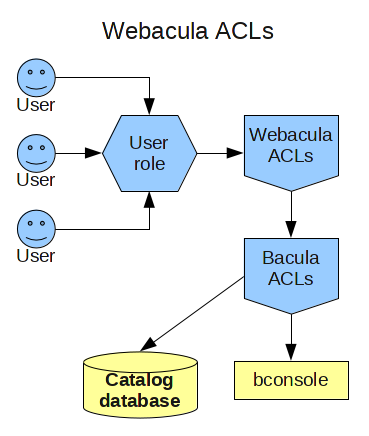
\includegraphics[totalheight=0.45\textheight,keepaspectratio=true]{./pics/ACLs.png}
  \caption[Webacula ACLs]{Webacula ACLs}
  \label{Webacula ACLs}
\end{figure}

If the user (more precisely --- a role) does not have any a ACL rule, that user has no rights.

ACL rules are applied in the order which is defined by field value ''order''.

Bacula and Webacula ACLs can conflict.
For example, usage of a Bacula command \texttt{status} is allowed to the user, 
but access to Webacula menu item \texttt{Director} at the same time is forbidden.

In this case the user sees the message like :
\begin{verbatim}
You try to use Webacula menu "director".
Webacula ACLs : Access denied.
\end{verbatim}

And on the contrary.
Access to Webacula menu item \texttt{Director} can be allowed. And usage of a Bacula command \texttt{status} can be forbidden.

In this case the user sees the message like :
\begin{verbatim}
You try to run Bacula Console with command "status".
Bacula ACLs : Access denied.
\end{verbatim}

\textbf{NOTE}.
Pay attention that in the first case access has been forbidden by a \textit{Webacula} ACL rule, 
and in the second a \textit{Bacula} ACL rule.


\subsection{Users and roles}
\label{Setup:Users and roles}

In Webacula the concept of users and roles is used.
Each user has the role. There is no user without a role.

In other words you should create a role at first, and then create the user and assign to it a certain role.

The role can inherit from other role.

After install, Webacula has two built in roles :

\begin{itemize}
  \item \textbf{root\_role} --- default built-in superuser role. 
  \item \textbf{operator\_role} --- typical built-in role for backup operator.
\end{itemize}

Users by whom the role \textbf{root\_role} is assigned are superusers, they have all rights to all.
This role cannot be deleted and the role name cannot be changed.

After installation \textbf{root\_role} is assigned to the user with a login name \textbf{root}.

The role \textbf{operator\_role} can fulfill any operations except of the administarators functions : 
creation, change, assignment of roles, users.



\section{Update from prior version}
\label{Update}

\textbf{IMPORTANT}. Now there is no separate Webacula database.
All Webacula tables are allocated in a Bacula database and have a prefix\texttt{ webacula\_}.

Therefore, if you conducted Webacula \textit{LogBook}, you need to take care to transfer \texttt{wbLogBook} table 
to a Bacula database in \texttt{webacula\_logbook} table.

Precisely also transfer the data from Webacula database \texttt{wbJobDesc} table 
to Bacula database to table \texttt{webacula\_jobdesc}.

From a file \texttt{config.ini} delete from \texttt{[webacula]} sections lines with the connection 
description to a Webacula database.

Also remove \texttt{tmpdir} from \texttt{config.ini}. Use 'data/' directory instead.

The script \texttt{webacula\_clean\_tmp\_files.sh} is not necessary now.


\end{document}